%% ----------------------------------------------------------------
%% Theory.tex
%% ---------------------------------------------------------------- 
\chapter{Theory} \label{Chapter: Theory}

%Check that you provide enough background information: your reader does not know what you know. Assuming that your reader knows much more than you and therefore omitting background information is a very common problem with students.

%Many students seem to think that they know little while everyone else knows a lot—therefore they shouldn’t explain things that everyone probably already knows. It is only later in their careers when they realise that no-one really knows that much! Besides, there will be readers from adjacent (sub)fields and readers who are just learning the tricks of the trade. Use a colleague who works on something slightly different than you as a test reader—ask her which parts of the text are hard to follow, and revise accordingly.

%\begin{enumerate}
%\item Setting the scene
%\item Underlying information
%\end{enumerate}

\section{Deep Learning}

%TODO: include parts of the literature review over here.

"Since then improvements have been made in part enabled by the access to greater computational resources, especially graphics processing units (GPU), enabling training of deep neural networks containing many parameters in reasonable time. Given this, specialized neural network architectures like convolutional neural networks (CNN) and recurrent neural networks (RNN) with long short-term memory cells (LSTM) can now be trained efficiently and have been successfully applied to many problems" \cite{Jurtz2017}

"Recently, Deep-Learning (DL) gained attention with applications in several domains, such as speech recognition systems (the first major industrial application of DL), natural language understanding, sentiment analysis, language translation, image recognition, particle accelerator data analysis and Bioinformatics. Here, it is important to recall that it was possible with the advent of the Graphical Processing Units (GPUs). DL approaches are representation-learning methods with multiple levels of representation, from the raw input to a slightly more abstract level [22]. Basically, a DL architecture is composed by a stack of modules that are subject to learning with a large number of parameters. Moreover, it is known that large networks rarely present local minima. However, such networks are prone to overfitting. Also, training different architectures is very hard because finding an optimal set of hyper-parameters for each architecture is a difficult task and training each network is computationally expensive.
[...]
The training of deep networks was proved to be hard due to the variation of the backpropagated gradients at each time step, typically vanishing over several time steps [22]. Regarding this issue, [24] proposed a way to explore the use of rectifying non-linearities instead of using the well- known sigmoid and hyperbolic tangent functions, known as the Rectified Linear Units (ReLU), which is a better model of biological neurons and allows the network to obtain sparse representations. Nowadays, the ReLU is considered to be the most popular non-linear activation function. It is a half-wave rectifier f(x) = max(x, 0) (where x is the input to a neuron). The advantage of the ReLU, compared with other logistic functions, is that it learns much faster in multi-layer networks, allowing training of a deep supervised network [22]." \cite{Hattori2017}

	\subsection{Convolutional Neural Networks}
	%TODO: include parts of the literature review over here.
	
	"In convolutional neural networks (CNNs) information also flows only from the input to the output, layer by layer. They are however not fully connected, but instead slide a filter (a set of weights) over the input that feeds into a different neuron in the next layer each time it is moved as illustrated in Figure 1B. The filter will thereby identify features in input irrespectively of where they appear. This concept is visualized in Figure 1C using the example of a convolutional filter detecting a motif in an amino acid sequence. Pooling such as mean pooling (averaging of nearby positions) enables the network to become invariant to small local de- formations in the input. Convolutional neural networks often consist of many convolutional filters and many convolutional and pooling layers to enable the network to integrate the information from the different filters and various levels of abstraction (LeCun et al.,2015). When applied to biological problems, convolutional neural networks are ideally suited to locate motifs, for example in a protein sequence, independent of their position within the sequence." \cite{Jurtz2017}
	
	"Max-pooling provides a way of reducing the input or hidden layer size by selecting only the maximally activated neuron from a number of neighboring neurons. Alternatively mean pooling can be performed where the mean activation is calculated among neighboring neurons. Pooling is often used in convolutional neural networks (LeCun et al., 2015). To make a convolutional neural network independent of the input sequence length, global max-pooling can be applied where only the maximally activated neuron of the input or hidden layer is selected for each of the convolutional filters. In this way, the number of hidden neurons generated by the convolutional filters is equal to the number of filters and not influenced by the input sequence length." \cite{Jurtz2017}
	
	"Each convolution layer consists of four consecutive operations: 1) The convolution operation with certain kernel size. 2) The batch normalization (Ioffe and Szegedy, 2015) operation is applied to help speed up
	the training process and acts as a regularizer. 3) The activation operation, ‘ReLU,’ (Radford et al., 2015) was used as an activation function. 4) The dropout (Srivastava et al., 2014) operation to prevent the neural network from overfitting randomly drops neurons during the deep network training process such that the network can avoid too much co-adapting." \cite{Fang2017}
	
	"The proposed Deep3I network (see Fig. 2) differs from the previous net- work (Li and Yu, 2016; Busia and Jaitly, 2017) in that the latter ones used residual blocks and multi-scale layer containing CNN layers with a convolution window size of 3, 7, and 9 to discover protein local and global context. Deep3I consists of stacked CNN layers, whose convolution window size is only 3. When stacked deep convolution blocks are put together, they can perform both local and global context extraction. Applying convolution on top of convolution, the sliding window will cover a wide range of protein sequences by using this hierarchical convolutional operation." \cite{Fang2017}
	\begin{figure}[h]
		\centering
		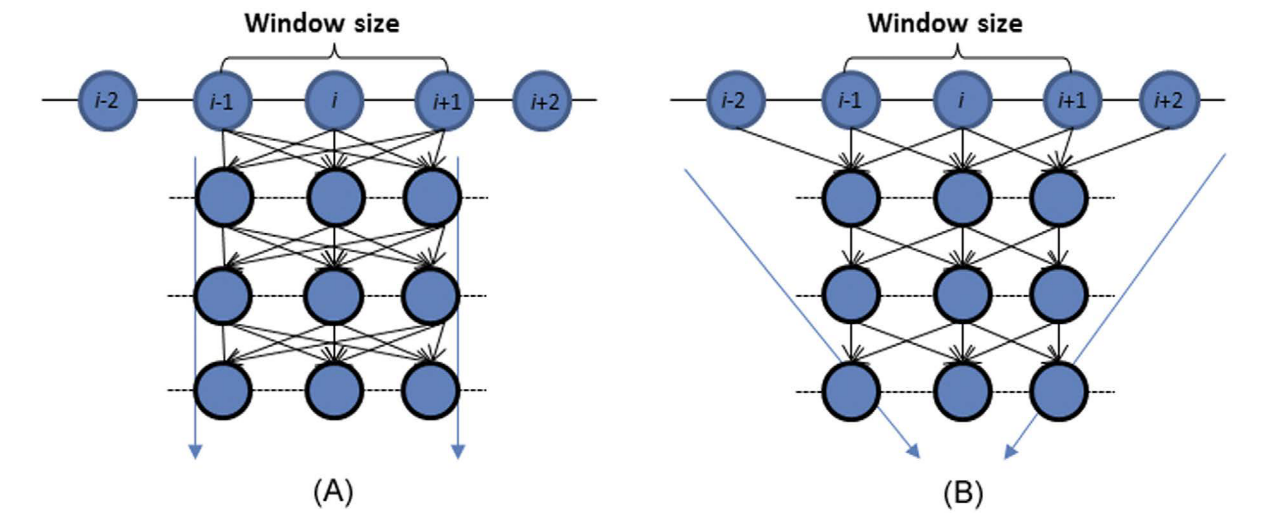
\includegraphics[width=1\linewidth]{cnnwang}
	\end{figure}
	
	"Although a fully-connected layer–where every input of interest is connected to every neuron in the layer by a distinct weight–is usually considered the simplest type of layer in a neural network, in some senses a convolutional layer can be thought of as a further simplification. Whereas fully-connected layers can be understood as an attempt to capture information from the inputs simultaneously by defining a large number of neurons with distinct weights, convolutional layers consist of filters–smaller groups of neurons– which look at segments of the input sequence at a time. Thus, a convolutional filter can be interpreted as sliding along the input sequence, reusing the same few weights on each local patch of the input. [...] The convolutional filters, CF and CF’, are defined by their width–the number of inputs examined at a time–and depth–the number of neurons in the filter. [...] one of the major benefits of convolutions compared to a the previous fixed-window, fully-connected approach: in situations where local properties of the data are critical, stacking small filters–each of which examines a small local input patch at a time–introduces the ability to learn and maintain information about sequence dependencies at different scales. [...] filters in lower layers focus on extracting information from small local contexts–in this case, of three residues–while filters in higher layers cover correlations which are more spatially spread-out in the input sequence." \cite{Busia2017}
	
	"Convolutional neural networks (CNN) [LeCun et al., 1998], a specific type of deep neural networks using translation-invariant convolutional kernels, can be applied to extracting local con- textual features and have proven to be effective for many natural language processing (NLP) tasks [Yih et al., 2011; Zhang et al., 2015]. Inspired by their success in text classification, in this paper, CNNs with various kernel sizes are used to extract multiscale local contexts from a protein sequence." \cite{Li2016}

\section{Interpretability techniques}

"There is a growing sense that neural networks need to be interpretable to humans. The field of neural network interpretability has formed in response to these concerns. As it matures, two major threads of research have begun to coalesce: feature visualization and attribution. 

\textbf{Feature visualization} answers questions about what a network — or parts of a network — are looking for by generating examples.

\textbf{Attribution} (or saliency maps) studies what part of an example is responsible for the network activating a particular way." \cite{Olah2017}

"One of the challenges of neural networks is understanding what exactly goes on at each layer.
We know that after training, each layer progressively extracts higher and higher-level features of the image, until the final layer essentially makes a decision on what the image shows.
For example, the first layer maybe looks for edges or corners.
Intermediate layers interpret the basic features to look for overall shapes or components, like a door or a leaf.
The final few layers assemble those into complete interpretations---these neurons activate in response to very complex things such as entire buildings or trees." \cite{Mordvintsev2015}

"Deep neural networks are highly expressive models that have recently achieved state of the art performance on speech and visual recognition tasks. While their expressiveness is the reason they succeed, it also causes them to learn uninterpretable solutions that could have counter-intuitive properties." \cite{Szegedy2013}

"Nonlinear methods such as Deep Neural Networks (DNNs) are the gold standard for various challenging machine learning problems, e.g., image classification, natural language processing or human action recognition. Although these methods perform impressively well, they have a significant disadvantage, the lack of transparency, limiting the interpretability of the solution and thus the scope of application in practice. Especially DNNs act as black boxes due to their multilayer nonlinear structure.
[...]
An interpretable classifier explains its nonlinear classification decision in terms of the inputs. For instance, in image classification problems, the classifier should not only indicate whether an image of interest belongs to a certain category or not, but also explain what structures (e.g. pixels in the image) were the basis for its decision (cf. Figure 1). This additional information helps to better assess the quality of a particular prediction, or to verify the overall reasoning ability of the trained classifier. Also, information about which pixels are relevant in a particular image, could be used for determining which region of the image should be the object of further anal- ysis. Linear models readily provide explanations in terms of input variables (see for example [19], [20]). However, because of the limited expressive power of these models, they perform poorly on complex tasks such as image recognition. Extending linear analysis techniques to more realistic nonlinear models such as deep neural networks, is therefore of high practicala relevance." \cite{Montavon2017}
\begin{figure}
	\centering
	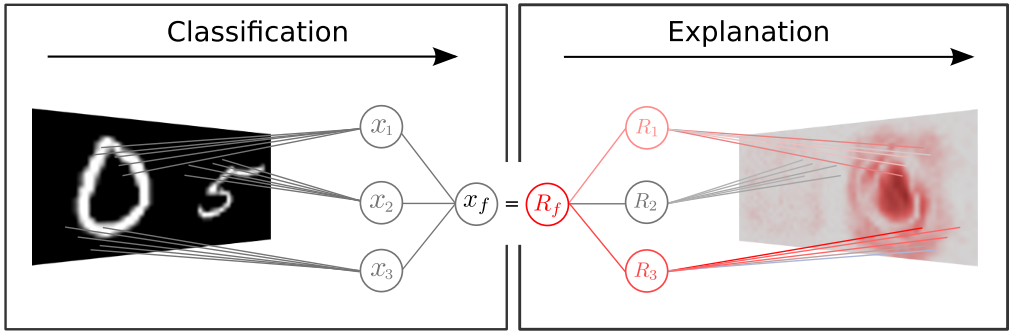
\includegraphics[width=0.7\linewidth]{deeptaylor}\\
\end{figure}

"Networks with Rectified Linear Units (ReLUs) create nonlinearities that must be addressed. Several variants exist for handling this [448,454]. Backpropagation-based methods are a highly active area of research. Researchers are still actively identifying weaknesses [455], and new methods are being developed to address them [219,456,457]. Lundberg and Lee [458] noted that several importance scoring methods including integrated gradients and LIME could all be considered approximations to Shapely values [459], which have a long history in game theory for assigning contributions to players in cooperative games." \cite{Ching2017}

"The purported “black box” nature of neural networks is a barrier to adoption in applications where interpretability is essential." \cite{Shrikumar2017}

	\subsection{Feature visualization}
	
	"While quantitative analyses and comparisons of such models exist, and visualizations of the first layer representations are common in the literature, one area where more work needs to be done is the qualitative analysis of representations learned beyond the first level. [...] Our aim was to explore ways of visualizing what a unit computes in an arbitrary layer of a deep network. The goal was to have this visualization in the input space (of images), to have an efficient way of computing it, and to make it as general as possible (in the sense of it being applicable to a large class of neural-network-like models)." \cite{Erhan2009}
	
		\subsubsection{Linear combination of filters}
		"Lee et al. (2008) showed one way of visualizing what the units in the second hidden layer of a network are responding to. They made the assumption that a unit can be characterized by the filters of the previous layer to which it is most strongly connected (i.e. whose weight to the upper unit is large in magnitude). By taking a weighted linear combination of the previous layer filters [...].
		Lee et al. (2009) used an extended version of this method for visualizing units of the third layer [...].
		Such a technique is simple and efficient. One disadvantage is that it is not clear how to automatically choose the appropriate number of filters to keep at each layer. [...], this method also bypasses the nonlinearities between layers" \cite{Erhan2009}
	
		\subsubsection{Activation maximization}
		"we look for input patterns of bounded norm which maximize the activation of a given hidden unit (The total sum of the input to the unit from the previous layer plus its bias.); since the activation function of a unit in the first layer is a linear function of the input, in the case of the first layer, this input pattern is proportional to the filter itself. [...] 
		One simple way of doing this is to find, for a given unit, the input sample(s) (from either the training or the test set) that give rise to the highest activation of the unit. Unfortunately, this still leaves us with the problem of choosing how many samples to keep for each unit and the problem of how to “combine” these samples. Ideally, we would like to find out what these samples have in common. Furthermore, it may be that only some subsets of the input vector contribute to the high activation, and it is not easy to determine which by inspection.
		[...]
		maximizing the activation of a unit as an optimization problem.
		\begin{equation}
		x* = arg \max\limits_{x \; s.t. ||x||=\rho} h_{ij}(\theta,x)
		\end{equation}
		This is, in general, a non-convex optimization problem. But it is a problem for which we can at least try to find a local minimum. This can be done most easily by performing simple gradient ascent in the input space [...] 
		the unit can then be characterized by the minimum or set of minima found. In the latter case, one can either average the results, or choose the one which maximizes the activation, or display all the local minima obtained to characterize that unit.
		This optimization technique (we will call it “activation maximization”) does involve a choice of hyperparameters: the learning rate and a stopping criterion" \cite{Erhan2009}
		
		"the response of an internal unit to input images, as a function in image space, appears to be unimodal, or at least that the maximum is found reliably and consistently for all the random initializations tested. This is interesting because finding this dominant mode is relatively easy, and displaying it then provides a good characterization of what the unit does." \cite{Erhan2009}
		
		"We tested the activation maximization procedure on image patches of 20 × 20 pixels (instead of 12×12) and found that the optimization does not converge to a single global minimum. Moreover, the input distribution that is sampled with the units clamped to 1 has many different modes and its expectation is not meaningful or interpretable any-more. [...] 
		It is perhaps unrealistic to expect that as we scale the datasets to larger and larger images, one could still find a simple representation of a higher layer unit. We should note, however, that there is a recent trend of developing convolutional versions of deep architectures (Kavukcuoglu et al., 2009; Lee et al., 2009; Desjardins \& Bengio, 2008): it is likely that one will be able to apply the same techniques in that scenario and still be able to recover good visualizations, even with large inputs." \cite{Erhan2009}
		
		"One way to visualize what goes on is to turn the network upside down and ask it to enhance an input image in such a way as to elicit a particular interpretation. Say you want to know what sort of image would result in “Banana.” Start with an image full of random noise, then gradually tweak the image towards what the neural net considers a banana (see related work in [1], [2], [3], [4]). By itself, that doesn’t work very well, but it does if we impose a prior constraint that the image should have similar statistics to natural images, such as neighboring pixels needing to be correlated." \cite{Mordvintsev2015}
		
		"Neural networks are, generally speaking, differentiable with respect to their inputs. If we want to find out what kind of input would cause a certain behavior --- whether that's an internal neuron firing or the final output behavior --- we can use derivatives to iteratively tweak the input towards that goal [3]." \cite{Olah2017}
		\begin{figure}[h]
			\centering
			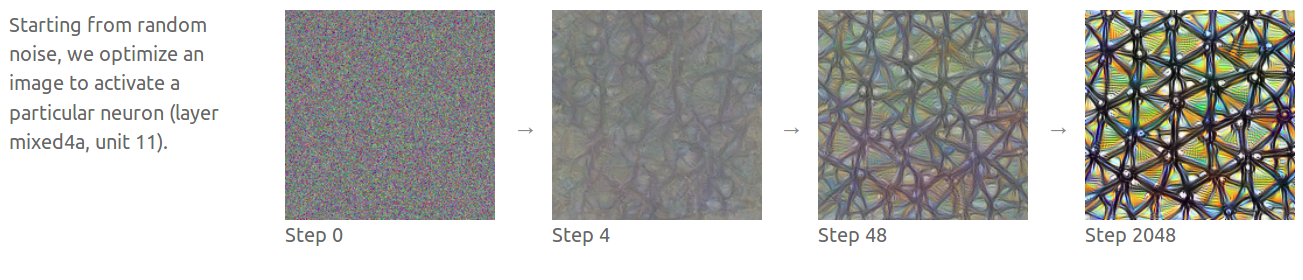
\includegraphics[width=1\linewidth]{randopt}
		\end{figure}
		
		" Optimization can give us an example input that causes the desired behavior --- but why bother with that? Couldn't we just look through the dataset for examples that cause the desired behavior?
		
		It turns out that optimization approach can be a powerful way to understand what a model is really looking for, because it separates the things causing behavior from things that merely correlate with the causes. [...] A neuron may not be detecting what you initially thought. Optimization also has the advantage of flexibility. For example, if we want to study how neurons jointly represent information, we can easily ask how a particular example would need to be different for an additional neuron to activate. This flexibility can also be helpful in visualizing how features evolve as the network trains. If we were limited to understanding the model on the fixed examples in our dataset, topics like these ones would be much harder to explore. " \cite{Olah2017}
		\begin{figure}[h]
			\centering
			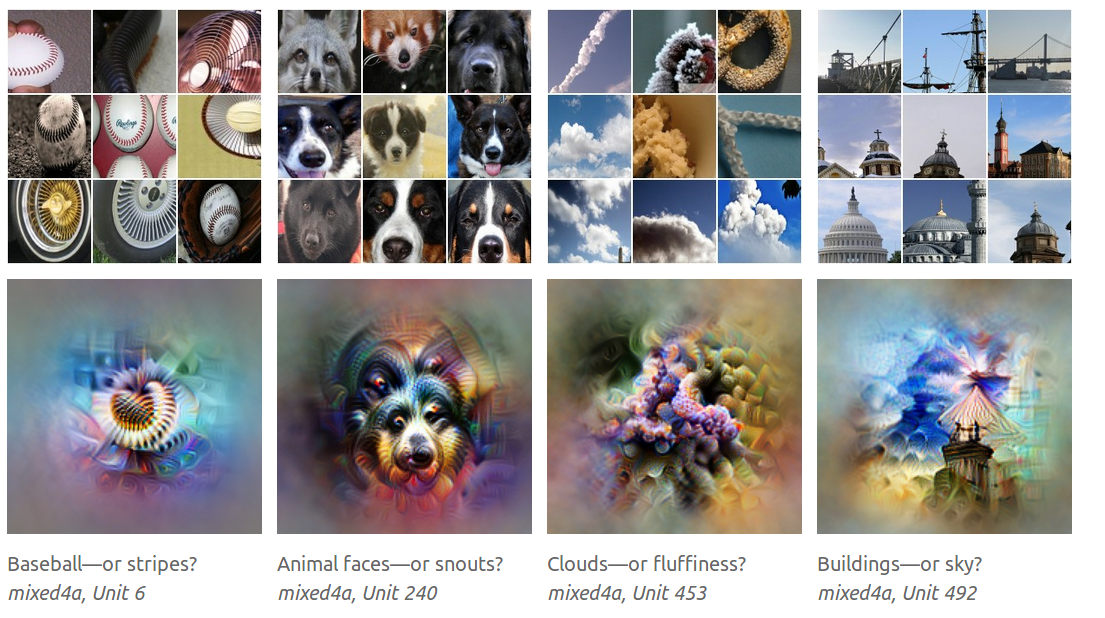
\includegraphics[width=1\linewidth]{optimization}
		\end{figure}
	
	\subsection{Saliency maps}
	"Bach et al. [22] have introduced the concept of pixel-wise decomposition of a classification decision, and how such decomposition can be achieved either by Taylor decomposition, or by a relevance propagation algorithm. Specifically, the authors distinguish between (1) functional approaches that view the neural network as a function and disregard its topology, and (2) message passing approaches, where the decomposition stems from a simple propagation rule applied uniformly to all neurons of the deep network.
	[...]
	the methods proposed in [27], [28] do not explain the decision of a classifier but rather perform sensitivity analysis by computing the gradient of the decision function. This results in an analysis of variations of that function, with- out however seeking to provide a full explanation why a certain data point has been predicted in a certain way. Specifically, the gradient of a function does not contain information on the saliency of a feature in the data to which the function is applied. Simonyan et al. [24] incorporate saliency information by multiplying the gradient by the actual data point.
	The method proposed by Zeiler and Fergus [21] was designed to visualize and understand the features of a convolutional neural network with max-pooling and rectified linear units. The method performs a backpropagation pass on the network, where a set of rules is applied uniformly to all layers of the network, resulting in an assignment of values onto pixels. The method however does not aim to attribute a defined meaning to the assigned pixel values, except for the fact that they should form a visually interpretable pat- tern. [22] proposed a layer-wise propagation method where the backpropagated signal is interpreted as relevance, and obeys a conservation property. The proposed propagation rules were designed according to this property, and were shown quantitatively to better support the classification decision [25]. However, the practical choice of propagation rules among all possible ones was mainly heuristic and lacked a strong theoretical justification" \cite{Montavon2017}
	
	"Shrikumar et al. and Kindermans et al. (Shrikumar et al., 2016; Kindermans et al., 2016) showed that absent modifications to deal with numerical stability, the original LRP rules were equivalent within a scaling factor to an elementwise product between the saliency maps of Simonyan et al. and the input (in other words, gradient × input)." \cite{Shrikumar2017}
	
	"Simonyan et al. [24] incorporate saliency information by multiplying the gradient by the actual data point." \cite{Montavon2017}
		
		\subsubsection{Perturbation-based forward propagation approaches (sensitivity analysis)}
		"To further test the robustness of the activation maximization method, we perform a sensitivity analysis in order to test whether the units are selective to these patterns found by the optimization routine, and whether these patterns strongly activate other units as well. The figure on the right shows the post-sigmoidal activation of unit j (columns) when the input to the network is the “optimal” pattern i (rows), found by our gradient procedure for unit i, normalized across columns in order to eliminate the effect of units that are activated for very many patterns in general. The strong values on the diagonal suggest that the results of the optimization have uncovered patterns that are mostly specific to a particular unit." \cite{Erhan2009}
		\begin{figure}[h]
			\centering
			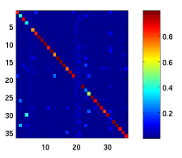
\includegraphics[width=0.2\linewidth]{sensitivity}
		\end{figure}
		
		"Simonyan et al. [24], however, demonstrated that DeConvNets can be interpreted as a sensitivity analysis of the network input/output relation." \cite{Mahendran2015}
		
		"the methods proposed in [27], [28] do not explain the decision of a classifier but rather perform sensitivity analysis by computing the gradient of the decision function. This results in an analysis of variations of that function, without however seeking to provide a full explanation why a certain data point has been predicted in a certain way. Specifically, the gradient of a function does not contain information on the saliency of a feature in the data to which the function is applied. Simonyan et al. [24] incorporate saliency information by multiplying the gradient by the actual data point." \cite{Montavon2017}
		
		"Zeiler and Fergus [36], who backtrack the network computations to identify which image patches are responsible for certain neural activations" \cite{Mahendran2015}
		
		"These approaches make perturbations to individual inputs or neurons and observe the impact on later neurons in the network. Zeiler \& Fergus (Zeiler \& Fergus, 2013) occluded different segments of an input image and visualized the change in the activations of later layers. “In-silico muta- genesis” (Zhou \& Troyanskaya, 2015) introduced virtual mutations at individual positions in a genomic sequence and quantified the their impact on the output. Zintgraf et al. (Zintgraf et al., 2017) proposed a clever strategy for analyzing the difference in a prediction after marginalizing over each input patch. However, such methods can be com- putationally inefficient as each perturbation requires a sep- arate forward propagation through the network. They may also underestimate the importance of features that have sat- urated their contribution to the output." \cite{Shrikumar2017}
		\begin{figure}[h]
			\centering
			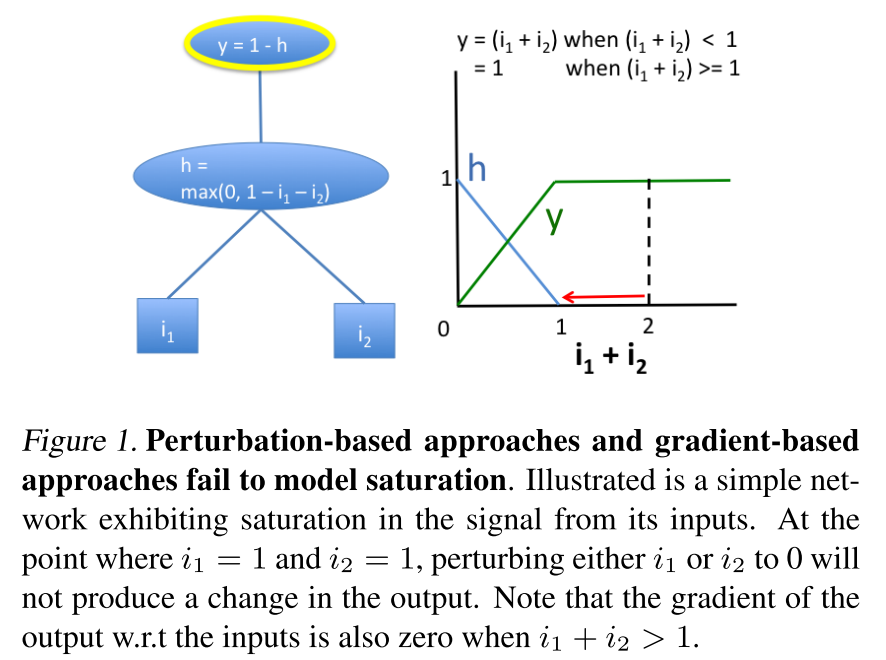
\includegraphics[width=0.6\linewidth]{saturation}
		\end{figure}

		\subsubsection{Backpropagation-based approaches}
		"In contrast to perturbation methods, backpropagation approaches are computationally efficient as they propagate an importance signal from the output neuron backwards through the layers towards the input in a single pass.
		DeepLIFT belongs to this family of approaches.
		[,,,]
		
		\textbf{GRADIENTS, DECONVOLUTIONAL NETWORKS AND GUIDED BACKPROPAGATION}
		Simonyan et al. \cite{Simonyan2014} proposed using the gradient of the output w.r.t. pixels of an input image to compute a “saliency map” of the image in the context of image classification tasks. The authors showed that this was similar to deconvolutional networks \cite{Zeiler2014} except for the handling of the nonlinearity at rectified linear units (ReLUs). When backpropagating importance using gradients, the gradient coming into a ReLU during the backward pass is zero’d out if the input to the ReLU during the forward pass is negative. By contrast, when backpropagating an importance signal in deconvolutional networks, the importance signal coming into a ReLU during the backward pass is zero’d out if and only if it is neg-ative, with no regard to sign of the input to the ReLU during the forward pass.
		Springenberg et al., (Springenberg et al., 2014) combined these two approaches into Guided Backpropagation, which zero’s out the importance signal at a ReLU if either the input to the ReLU during the for-ward pass is negative or the importance signal during the backward pass is negative. Guided Backpropagation can be thought of as equivalent to computing gradients, with the caveat that any gradients that become negative during the backward pass are discarded at ReLUs. Due to the zeroing out of negative gradients, both guided backpropagation and deconvolutional networks can fail to highlight inputs that contribute negatively to the output. Additionally, none of the three approaches would address the saturation problem illustrated in Fig. 1, as the gradient of y w.r.t. h is negative (causing Guided Backprop and deconvolutional networks to assign zero importance), and the gradient of h w.r.t both i1 and i2 is zero when i1 + i2 > 1 (causing both gradients and Guided Backprop to be zero). Discontinuities in the gradients can also cause undesirable artifacts." \cite{Shrikumar2017}
		\begin{figure}[h]
			\centering
			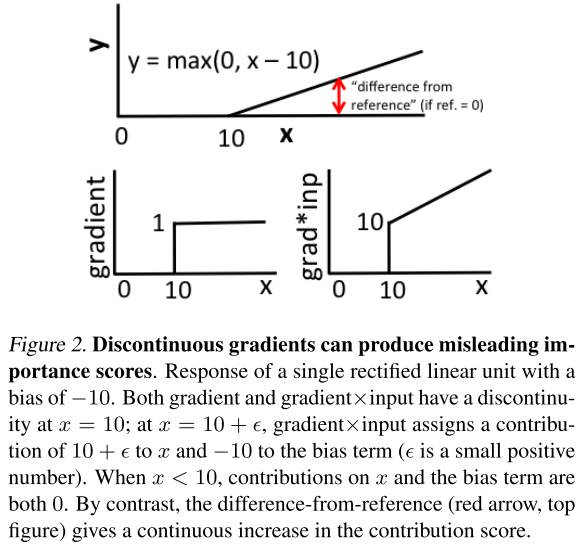
\includegraphics[width=0.6\linewidth]{discontinuity}
		\end{figure}
		
		\textbf{LAYERWISE RELEVANCE PROPAGATION AND GRADIENT × INPUT}
		"Bach et al. (Bach et al., 2015) proposed an approach for propagating importance scores called Layerwise Relevance Propagation (LRP).
		
		Shrikumar et al. and Kindermans et al. (Shrikumar et al., 2016; Kindermans et al., 2016) showed that absent modifications to deal with numerical stability, the original LRP rules were equivalent within a scaling factor to an elementwise product between the saliency maps of Simonyan et al. and the input (in other words, gradient × input).
		[...]
		While gradient × input is often preferable to gradients alone as it leverages the sign and strength of the input, it still does not address the saturation problem in Fig. 1 or the thresholding artifact in Fig. 2." \cite{Shrikumar2017}
		
		\textbf{INTEGRATED GRADIENTS}
		"Instead of computing the gradients at only the current value of the input, one can integrate the gradients as the inputs are scaled up from some starting value (eg: all zeros) to their current value (Sundararajan et al., 2016). This ad- dressess the saturation and thresholding problems of Fig. 1 and Fig. 2, but numerically obtaining high-quality inte- grals adds computational overhead. Further, this approach can still give highly misleading results (see Section 3.4.3)." \cite{Shrikumar2017}
		
		\textbf{DeepLIFT}
		"Our approach is unique in two regards: first, it frames the question of importance in terms of differences from a ‘reference’ state, where the ‘reference’ is chosen by the user according to what is appropriate for the problem at hand. In contrast to most gradient-based methods, using a difference-from-reference allows DeepLIFT to propagate an importance signal even in situations where the gradient is zero and avoids artifacts caused by discontinuities in the gradient. Second, by optionally giving separate consideration to the effects of positive and negative contributions at nonlinearities, DeepLIFT can reveal dependencies missed by other approaches. As DeepLIFT scores are com- puted using a backpropagation-like algorithm, they can be obtained efficiently in a single backward pass through the network after a prediction has been made." \cite{Shrikumar2017}
		
		\textbf{Deep Taylor Decomposition}
		"The main goal of this paper is to reconcile the functional and rule-based approaches for obtaining these decompositions, in a similar way to the error backpropagation algorithm [23] that also has a functional and a message passing interpretation. We call the resulting framework deep Taylor decomposition. This new technique seeks to replace the analytically intractable standard Taylor decomposition problem by a multitude of simpler analytically tractable Taylor decompositions—one per neuron.
		[...]
		Our method is based on deep Taylor decomposition and efficiently utilizes the structure of the network by backpropagating the explanations from the output to the input layer.
		[...]
		In this paper, we focus instead on the interpretation of the prediction of individual data points, for which portions of the trained model may either be relevant or not relevant.
		[...]
		The classification decision is first decomposed in terms of contributions R1, R2, R3 of respective hidden neurons x1, x2, x3, and then, the contribution of each hidden neuron is independently redistributed onto the pixels, leading to a relevance map (or heatmap) in the pixel space, that explains the classification “0”.
		A main result of this work is the observation that application
		of deep Taylor decomposition to neural networks used for image classification, yields rules that are similar to those proposed by [22] (the αβ-rule and the ?-rule), but with specific instantiations of their hyperparameters, previously set heuristically." \cite{Montavon2017}


\section{Deep Learning in biology}

%TODO: Include some parts of literature review over here.

"slowly spreading into biology and bioinformatics. One potential cause of this is the lack of examples or code templates tailored to bioinformatics problems combined with the notion that the implementation and training of deep learning methods is complicated and computationally challenging" \cite{Jurtz2017}

 \subsection{CNNs on biological sequence data}

 DeepCNF uses 2D convolutions with filters of size window times feature vector size.

 "Amino Acids C, A, D, A, D are encoded as ‘one-hot’ vectors with a 1 at the position corresponding to the amino acid type (A, C or D), and zero otherwise. A filter (blue) is slid over the input sequence. The filter here has a length of three amino acids. At each position the filter has a preference for different amino acid types. The filter output is calculated by taking the sum of the element-wise product of the input and the filter position-specific weights. Each time the filter is moved, it feeds into a different hidden neuron in the hidden layer, here visualized in the f1 row. Multiple filters will give multiple inputs to the next layer {f1, f2, f3, ...}. A filter can be visualized as a sequence motif. This helps to understand which amino acids the filter prefers at each sequence position. When the filter is slid over the input sequence, it functions as motif detector and becomes activated when the input matches its preference. For example, this filter has negative output for sub-sequences ADC and positive for DCD." \cite{Jurtz2017}
 \begin{figure}[h]
	\centering
	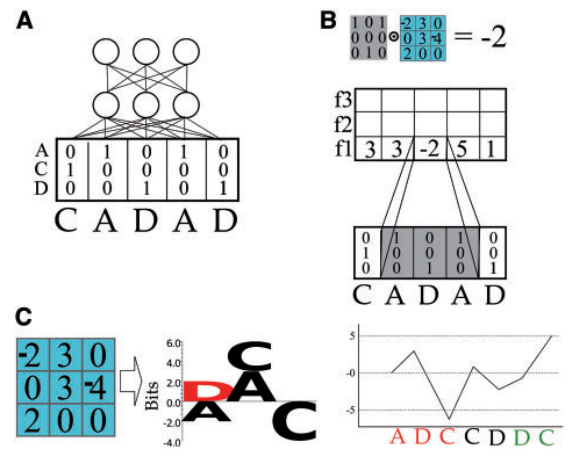
\includegraphics[width=0.7\linewidth]{cnnbio}
 \end{figure}
		
 "Convolutional Neural Networks (CNNs) have been used to overcome the limitations of windowing by applying layers of shifting convolutional kernels across the input sequence (Wang et al., 2016). The addition of each subsequent convolutional layer includes a window of information from the layer prior. This has the effect of growing the size of the window being applied to the input data, each time a layer is added. However, even though the effective window size increases at each layer, the total window is still finite and limited. DeepCNF for example uses five CNN layers, each with a window size of 11 (five on either side), this is only able to capture information from residues plus or minus 25 sequence positions away." \cite{Heffernan2017}

 \subsection{Interpretability techniques on biological problems}
 "In recent years, there has been an explosion of deep learning models which have lead to groundbreaking results in many fields such as computer vision[13], natural language processing[25], and computational biology [2, 19, 27, 11, 14, 22]. However, although these models have proven to be very accurate, they have widely been viewed as “black boxes” due to their complexity, making them hard to understand. This is particularly unfavorable in the biomedical domain, where understanding a model’s predictions is extremely important for doctors and researchers trying to use the model.
  [...]
 While making accurate predictions is important in biomedical tasks, it is equally important to understand why models make their predictions. Accurate, but uninterpretable models are often very slow to emerge in practice due to the inability to understand their predictions, making biomedical domain experts reluctant to use them. Consequently, we aim to obtain a better understanding of why certain models work better than others, and investigate how they make their predictions by introducing several visualization techniques.
  [...]
 The main difference between our work and previous works on images and natural language is that instead of trying to understand the DNNs given human understanding of such human perception tasks, we attempt to uncover critical signals in DNA sequences given our understanding of DNNs." \cite{Lanchantin2016}

	\subsubsection{Feature visualization}
	"The networks whose filters were saved and plotted only used one-hot encoding so as to be able to represent all features as PSSM-logos. The visualization of the convolutional filters was based on the methodology used in [37]. The convolutional filters are represented as a matrix of filter\_width columns and aa\_encoding rows. So as to visualize the relative importance of each of the positions in the filter, each of them is rescaled in a way that the height of the highest column is 1. After this transformation, each filter can be visualized as a PSSM logo where the position importance is proportional to the height of the column and the height of each letter is proportional to the importance of the amino acid in that position. Seq2logo [42] is used in order to generate the PSSM-logo plots. The Seq2Logo default amino acid colour coding is used: negatively charged (DE) residues are red, polar uncharged residues (NQSGTY) are green, positively charged (RKH) residues are blue and the remaining are black." \cite{Fontal2017}

	"For TFBS prediction, Alipanahi et al.[2] was the first to implement a visualization method on a DNN model. They visualize their CNN model by extracting motifs based on the input subsequence corresponding to the strongest activation location for each convolutional filter (which we call convolution activation). Since they only have one convolutional layer, it is trivial to map the activations back, but this method does not work as well with deeper models. We attempted this technique on our models and found that our approach using saliency maps outperforms it in finding motif patterns (details in section 4). Quang and Xie [19] use the same visualization method on their convolutional-recurrent model for noncoding variant prediction." \cite{Lanchantin2016}

	"In the case of the NN trained in this project, where the inputs are protein sequences encoded as one-hot vectors, the optimized inputs lose the one-hot vector encoding but can be forced to behave as a Position Probability Matrix (PPM) which can then be represented as a motif. Formally, the following equation, where Si is the score (defined as the unscaled values for class Ci pre Softmax transformation) and X is the input sequence, is optimized:
	arg max Si(X) + λ ? X ?2 2.
	λ is the regularisation parameter. The L2-regularization term is introduced in order to minimize the number of significant amino acids per position in the optimized input sequence. The score used is the value of the pre-Softmax layer because the post-Softmax value can be maximized by just minimizing the scores of the other classes, and the objective is to get an ideal input for the desired class, not an input modified to score low in the remaining classes." \cite{Fontal2017}
	
	"Now we introduce an approach to extract a class-specific visualization for a DNN model, where we attempt to find the best sequence which maximizes the probability of a positive TFBS, which we call class optimization. Formally, we optimize the following equation where S+(X) is the probability (or score) of an input sequence X (matrix in our case) being a positive TFBS computed by the softmax equation of our trained DNN model for a specific TF:
	arg maxS+(X) + λ?X?2 2
	where λ is the regularization parameter. We find a locally optimal X through stochastic gradient descent, where the optimization is with respect to the input sequence. In this optimization, the model weights remain unchanged. This is similar to the methods used in Simonyan et al.[21] to optimize toward a specific image class. This visualization method depicts the notion of a positive TFBS class for a particular TF and is not specific to any test sequence." \cite{Lanchantin2016}
	
	"In order to focus on higher probable regions of the input space, the 2-norm regularizer can be replaced by a data density model p(x) which is called “expert” by Montavon et al.(2017). This leads to the following optimization problem:
	max x log p(ωc|x) + log p(x).
	Here, the prototype is encouraged to simultaneously produce strong class response and to  resemble  the  data.   By  application  of  Bayes’  rule,  the  newly  defined  objective  can  be identified, up to modeling errors and a constant term, as the class-conditioned data density p(x|ωc).  The learned prototype thus corresponds to the most likely input x for the class ωc.  A possible choice for the expert is the Gaussian Restricted Boltzmann Machine (RBM).
	The RBM is a two-layer, bipartite, undirected graphical model with a set of binary hidden units p(h), a set of (binary or real-valued) visible units p(v), with symmetric connections between the two layers represented by a weight matrix W.  The probabilistic semantics for an RBM is defined by its energy function" \cite{Montavon2018}
	
	\subsubsection{Saliency maps}
		\textbf{Signal masking approach}
		"This method was developed along the course of the project in order to evaluate the effect of removing the signal from certain regions of the input sequences. It is a way of assessing, for a trained model, which parts of the input sequence have a higher importance to determine the final classification." \cite{Fontal2017}
		
		\textbf{Gradient-based approach}
		"Our first visualization method is finding a test sequence’s saliency map which uses first-order derivatives to describe the importance of each nucleotide in making the final prediction. [...] we seek to visualize the influence of each position (i.e. nucleotide) on the prediction. Our approach is similar to the methods used on images by \cite{Simonyan2014} and Baehrens et al.[4]. Given a sequence X0 of length |X0|, and class c ∈ C, a DNN model provides a score function Sc(X0). We rank the nucleotides of X0 based on their influence on the score Sc(X0). Since Sc(X) is a highly non-linear function of X with deep neural nets, it is hard to directly see the influence of each nucleotide of X on Sc. Mathematically, around the point X0, Sc(X) can be approximated by a linear function by computing the first-order Taylor expansion:
		Sc(X) ≈ wTX + b = ?|X| wixi + b
		where w is the derivative of Sc with respect to the sequence variable X at the point X0:
		w =∂Sc∂X|X0 = saliency map
		This derivative is simply one step of backpropagation in the DNN model, and is therefore easy to compute. We do a pointwise multiplication of the saliency map with the one-hot encoded sequence to get the derivative values for the actual nucleotide characters of the sequence (A,T,C, or G) so we can see the influence of the character at each position on the output score. Finally, we take the element-wise magnitude of the resulting derivative vector to visualize how important each character is regardless of derivative direction. We call the resulting vector a “saliency map[21]” because it tells us which nucleotides need to be changed the least in order to affect the class score the most. As we can see from equation 5, the saliency map is simply a weighted sum of the input nucleotides, where the each weight, wi, indicates the influence of that nucleotide position on the output score.
		[...]
		From each positive test sequence (thus, 500 total for each TF dataset) we extract a motif from the saliency map by selecting the contiguous length-9 subsequence that achieves the highest sum of contiguous length-9 saliency map values." \cite{Lanchantin2016}
		
			
	

\section{Secondary Structure Prediction}

%TODO: Read through \cite{Wang2016}'s bibliography 1-12 and improve this section + add references.

Soon after they have been formed, proteins fold into 3D structures that primarily determine their function in the cell. Protein functions are of great value for the medical field, as their knowledge can help drug design, disease treatment, or early diagnosis.
However, due to the molecular scale, these structures cannot be easily measured, and any attempt to do so remains costly. A more feasible alternative is utilizing computational tools to predict protein structures from amino-acid sequences alone, as these can be easily obtained from DNA sequencing and they are widely available on heavily annotated public databases. \cite{Hattori2017} points out that from the nearly 85 millions proteins whose sequences are known, we only know the structure of about 130 thousands.

(Dill and MacCallum, 2012)
"it is a problem which has remained unsolved since its inception half a century ago (Gibson and Scheraga, 1967)" \cite{Heffernan2017}
"site-specific mutation experiments (Drozdetskiy et al., 2015)." \cite{Fang2017}
"Accurately and reliably predicting structures, especially 3D structures, from protein sequences is one of the most challenging tasks in computational biology, and has been of great interest in bioinformatics [Ashraf and Yaohang, 2014]."\cite{Li2016}
(Yaseen and Li, 2014)

3D protein structure prediction from the sequence is a rather complex task, and thus researchers have focused firstly on the prediction of the so-called secondary structure, which consists on detecting local structures that can be used later for an easier modelling of the tertiary (3D) structure. Broadly, there are three kinds of local structures: $\alpha$-helix, $\beta$-sheet, and coil, which includes everything else. A finer classification schema developed by DSSP comprehends eight classes, three helices, two sheets, and three coils.

(Kabsch and Sander, 1983)
"Secondary structure prediction can be dated back to 1951 when Pauling and Corey proposed helical and sheet conformations of protein backbone based on hydrogen bonding patterns (Pauling et al.,1951)." \cite{Heffernan2017}
"This hypothesis has driven a decades-long effort, spanning multiple disciplines, to deduce how protein sequence determines a protein’s structural and functional properties (Dill et al., 2008; Anfinsen, 1977)." \cite{Busia2017}

"After translation, proteins fold into a 3-dimensional structure, known as the tertiary structure (Fig. 3A)."\cite{Jurtz2017}
"The 3D structure of a protein is determined largely by its amino acid sequence1." \cite{Wang2016}
"Knowledge of a protein’s structure can help to understand its function. Therefore de novo prediction of protein structure from sequence is a problem of great biological interest (Dill and MacCallum, 2012)." \cite{Jurtz2017}
"However it is extremely challenging to predict protein structure from sequence alone2." \cite{Wang2016}
"An important step in the prediction of tertiary protein structure is the prediction of the secondary structure, the local conformations of the peptide back-bone." \cite{Jurtz2017}
"There are three main classes of secondary structure: alpha-helix, beta-strand and coil. These can be further divided into 8 classes (Kabsch and Sander, 1983) (3 sub-classes of helix, 2 sub-classes of strands and 3 sub-classes of coil)." \cite{Jurtz2017}
"Since protein structure is critical to analysis of its function and many applications like drug and/or enzyme design3–5, understanding the complex sequence-structure relationship is one of the greatest challenges in computational biology6–8. Accurate protein structure and function prediction relies, in part, on the accuracy of secondary structure prediction9–12. [...] Overall, protein secondary structure can be regarded as a bridge that links the primary sequence and tertiary structure and thus, is used by many structure and functional analysis tools15–18" \cite{Wang2016}
"Protein tertiary structure prediction from amino acid sequence is a very challenging problem in computational biology (Yaseen and Li, 2014; Dill and MacCallum, 2012). However, if a protein secondary structure can be predicted accurately, it can provide useful constraints for 3D protein structure prediction. Protein secondary structure can also help identify the protein function domains and may guide the rational design of site-specific mutation experiments (Drozdetskiy et al., 2015)." \cite{Fang2017}
"The three-dimensional structure is also known as native conformation and it is a function of its secondary structures. A number of diseases, including cancer, Alzheimer’s disease, cystic fibrosis, Huntington’s disease and diabetes are linked to the result of the aggregation of ill-formed proteins [1], [2]. Notwithstanding, despite a large number of proteins that have been discovered recently (around 84.8 million records in the UniProtKB/TrEMBL repository as in may/2017), only a few of them have their structure known (129,745 in the Protein Data Bank – PDB as in may/2017). Therefore, acquiring knowledge about the structure of proteins is an important issue, since such knowledge can lead to important medical and biochemical advancements and even to the development of new drugs with specific functionality [3], [2]. [...] A possible way to infer the full structure of an unknown protein is to determine secondary structures in it. However, the pattern formation rules of secondary structures of proteins are still not known precisely [3]." \cite{Hattori2017}
"Proteins perform a wide variety of molecular functions, and most of those functions are determined by the protein’s three-dimensional structures. The problem of predicting the three-dimensional structure of a protein, given only its linear sequence of residues, is crucially important due to the high cost of experimental protein structure determination and the low cost of DNA sequencing to obtain protein sequences. However, even with this importance it is a problem which has remained unsolved since its inception half a century ago (Gibson and Scheraga, 1967; Dill and MacCallum, 2012; Zhou et al., 2011). Due to the challenge of predicting three-dimensional protein structure, the problem is commonly divided into smaller, more achievable problems, in the hopes that their solutions will ultimately lead to the solution for three-dimensional structure prediction. One type of these sub-problems is the prediction of one-dimensional structural properties of proteins, which can be represented as a one-dimensional vector along the protein sequence. The most commonly predicted one-dimensional structure of proteins is secondary structure. Secondary structure prediction can be dated back to 1951 when Pauling and Corey proposed helical and sheet conformations of protein backbone based on hydrogen bonding patterns (Pauling et al.,1951). Secondary structure is a course-grained descriptor of the local structure of the polypeptide backbone." \cite{Heffernan2017}
"Protein-based interactions are responsible for controlling a variety of vital functions: they are critical in driving the immune system, regulating breathing and oxygenation, controlling aging and energy usage, and determining drug response, with a protein’s particular functional role determined by its structure (Breda et al., 2006; Guo, Ellrott, \& Xu, 2008). Over time, scientists have reached a consensus that a protein’s structure primarily depends on its amino acid sequence–local and long-range interactions between amino acid residues and their side-chains are both a cause and consequence of protein secondary and tertiary structure (Dill et al., 2008). This hypothesis has driven a decades-long effort, spanning multiple disciplines, to deduce how protein sequence determines a protein’s structural and functional properties (Dill et al., 2008; Anfinsen, 1977).
As the number of proteins with known sequence continues to outpace the number of experimentally determined secondary and tertiary structures (Huang, Liu, \& Weinberger, 2016), computational approaches to protein structure prediction become increasingly desirable. Computational tools that can handle large amounts of data while making sufficiently accurate predictions of secondary structures can potentially serve to mitigate the cost and time burden in the experimental determination of protein structures." \cite{Busia2017}

"There is a natural upper-bound on the maximum possible Q3 accuracy from inconsistencies in secondary structure assignment likely due to the coarseness and inherent arbitrariness of three-class labels (Kihara, 2005). This is likely also the case for the eight-class instantiation of the problem. A better approach might be to predict the sequence of back-bone angles for the amino acids, since these are experimentally observed values." \cite{Busia2017}

"Accurately and reliably predicting structures, especially 3D structures, from protein sequences is one of the most challenging tasks in computational biology, and has been of great interest in bioinformatics [Ashraf and Yaohang, 2014]. Structural understanding is not only critical for protein analysis, but also meaningful for practical applications including drug design [Noble et al., 2004]. Understanding protein secondary structure is a vital intermediate step for protein structure prediction as the secondary structure of a protein reflects the types of local structures (such as 310−helix and β−bridge) present in the protein. Thus, an accurate secondary structure prediction significantly reduces the degree of freedom in the tertiary structure, and can give rise to a more precise and high resolution protein structure prediction [Ashraf and Yaohang, 2014; Zhou and Troyanskaya, 2014; Wang et al., 2011]." \cite{Li2016}

 \subsection{Features}
 "The input features we used are the same as (Busia and Jaitly, 2017). The amino acid at position i is represented as one-hot vector. There are 20 different types of amino acids. Some special amino acid cases were handled as follows: Amino Acid ‘X’ was treated as amino acid ‘A’. ‘B’ was treated as amino acid ‘N’. ‘Z’ was treated as amino acid ‘Q’. Since the input size was fixed at 700, if the input protein sequences were less than 700 amino acids; the remaining amino acid positions were padded with the ‘NoSeq’ label, which means no amino acid was there. Current implementation can handle any protein sequence length less or equal to 700 amino acids. The protein sequences will be split into smaller segments if they have more than 700 amino acids. [...] The profile information is also represented as 700-by-21 array. Hence, the input dimension is 700-by-42 in total." \cite{Fang2017}

 "each amino acid (ai) of the sequence (with n amino acids) has 42 features: 22 profile features are used for representing scores obtained from a Position-Specific Scoring Matrix (PSSM) [21], which are normalized using the logistic Sigmoid function. The last 20 features are used for representing the amino acid, using the one-hot encoding. In this encoding, only one bit is set and represents the name category of the amino acid." \cite{Hattori2017}

 "amino acid was encoded using one-hot encoding and additionally a sequence profile." \cite{Jurtz2017}

 "the first set of predictors take seven representative physio-chemical properties (PP) of amino acids (Fauche`re et al., 1988), 20-dimensional Position Specific Substitution Matrices (PSSM) from PSI-BLAST (Altschul et al., 1997), and 30-dimensional hidden Markov Model sequence profiles from HHBlits (Remmert et al., 2012) per residue as input [...] These features were selected previously in the development of SPIDER for secondary structure and contact prediction (Lyons et al., 2014; Heffernan et al., 2016, 2015). [...] The outputs from iteration 1 are then added to the PSSM, PP and HMM profile features, as inputs to a second set of predictors (iteration 2). This process is repeated two more times (iterations 3 and 4), for a total of four sets of networks as the result converges. [...] The TR4950 set is split into the same 10 folds for training every iteration of the network." \cite{Heffernan2017}

 "Each protein is represented as a sequence of amino acids, padded if necessary by no-sequence tokens to a sequence length of 700 residues. In turn, each amino acid is encoded as a 42-dimensional vector: the first twenty-one dimensions represent the one-hot encoding of the residue’s identity (or the no-sequence token), while the remaining dimensions contain Position-Specific Scoring Matrices (PSSM) generated with PSI-BLAST (see Zhou\&Troyanskaya (2014) for more details) which we normalize via mean-centering and scaling by the standard deviation." \cite{Busia2017}

 "Overtime, scientists have reached a consensus that a protein’s structure primarily depends on its amino acid sequence and concluded that the local and long-range interaction are a cause of protein second and tertiary structure. Based on this hypothesis, we can deduce that proteins with similar amino acid sequence tend to have similar secondary structure sequence. Therefore, the common sequence information contained by PSSM can contribute to the secondary structure prediction. For a protein with length L, PSSM is usually represented as a matrix with L ×21 dimensions where 21 denotes the 20 standard types of residues and one extra residue type which represents all non-standard residue types. Before PSSMs are used in- puts for CNNH\_PSS, they need to be transformed to 0–1 range by the sigmoid function. By concatenating sequence features and evolutional information, each residue in protein sequences can be encoded by a feature vector with dimension of 42." \cite{Zhou2018}
  \subsubsection{Beyond one-hot}
  "the input feature sequence X is decomposed into two parts, one is a sequence of 21-dimensional feature vectors encoding the types of the amino acids in the protein and the other is a sequence of 21-dimensional profile features obtained from the PSI-BLAST [Altschul et al., 1997] log file and rescaled by a logistic function [Jones, 1999]. Note that each feature vector in the first sequence is a sparse one-hot vector, i.e., only one of its 21 elements is none-zero, while a profile feature vector has a dense representation. In order to avoid the in- consistency of feature representations, we adopt an embed- ding operation from natural language processing to transform sparse sequence features to a denser representation [Mesnil et al., 2015]. This embedding operation is implemented as a feedforward neural network layer with an embedding matrix, Wemb ∈ R21×Demb, that maps a sparse 21-dimensional vector into a denser Demb-dimensional vector. In this paper, we empirically set Demb = 50, and initialize the embedding matrix with random numbers. The embedded sequence feature vector is concatenated with the profile feature vector before being fed into multiscale CNN layers." \cite{Li2016}

  "As the dimension of amino acid representation is already low, we only calculate a real value for every dimension by embedding technique and don’t decrease the dimension. The residue embedding in this paper is implemented by a feedforward neural net- work layer before multi-scale CNN in CNNH\_PSS [42]." \cite{Zhou2018}

  "The protein sequence input is one-hot vector, which is a sparse matrix. In the future work, ProtVec (Asgari and Mofrad, 2015) will be explored to represent the sequence so that it will become a much denser and picture-like matrix, which may improve the Q3 and Q8 accuracy." \cite{Fang2017}

 \subsection{PSI-BLAST profiles}
 "PSI-BLAST generates a PSSM of size T × 20 for a T lengthed sequence, where a higher score represents a higher likelihood of the ith amino acid replacing the current one in other species. Generally, two amino acids that are interchangeable in the PSSM indicates that they are also interchangeable in the protein without sig- nificantly modifying the functionality of the protein." \cite{Lin2016}

 "The BLOSUM matrix captures information about which pairs of amino acids are eas- ily interchangeable during evolution, but it does not capture information about the evolutionary constraints on a protein family (i.e. which amino acid positions are highly conserved and which are variable). This information can effectively be captured in a sequence profile. A sequence profile has the dimensions protein length times the number of amino acids and is conventionally generated by run- ning PSI-BLAST (Altschul et al., 1997) against a reference database. Encoding protein sequences as such profiles has demonstrated very helpful for prediction of for instance secondary structure (Jones, 1999)." \cite{Jurtz2017}

 "DeepCNF has no significant advantage over the others when a protein under prediction has very sparse sequence profile (i.e., Neff ≤ 2). That is, it is still challenging to predict SS structure from primary sequence instead of sequence profile." \cite{Wang2016}

 "We used the input features described in36. In particular, for each protein sequence, we ran PSI-BLAST41 with E-value threshold 0.001 and 3 iterations to search UniRef9079 to generate the position specific scoring matrix (PSSM). We then transform PSSM by the sigmoid function 1/(1 + exp(− x)) where x is a PSSM entry. We also use a binary vector of 21 elements to indicate the amino acid type at position i. We use 21 since there might be some unknown amino acids in a protein sequence. In total there are 42 input features for each residue, 21 from PSSM and the other 21 from the primary sequence. Note that besides using PSSM generated by 3 iterations, we could also add the PSSM generated by 5 iterations into the input features." \cite{Wang2016}

 "A protein sequence is represented as a 700-by-21 array in the system. Next, protein profiles were generated using PSI- BLAST (Altschul et al., 1997), as performed in some previous work (Wang et al., 2016; McGuffin et al., 2000). The PSI-BLAST tool param- eters were set as follows: evalue: 0.001, num\_iterations: 3, db, and UniRef50 to generate a position-specific scoring matrix (PSSM). PSSM is then transformed by the sigmoid function so that the value is in range (0,1)." \cite{Fang2017}

 "profile search time is relatively shorter than current available tools because we used a filtered version of the UniRef50 database. [...]
 The PSI-BLAST can generate the protein sequence profile in a short time if the search database is small, while a larger search database takes a longer time to get the profile and the prediction accuracy may not always increase. [...] Four different databases were downloaded from UniProt (http://www.uniprot.org/downloads). They are Swiss\_Prot (0.08GB), UniRef50 (4.3GB), UniRef90 (12GB) and UniRef100 (25GB). Take the UniRef50 database as an example: This database was used to perform a PSI-BLAST search with the parameter setup of evalue 0.001 and num\_iterations 3 on all protein sequences in the JPRED data set. Then, the train-ing set was used to train the Deep3I network, and the test set was used to report Q3, as shown in Table 1. The UniRef50 yielded the best results as a larger database was not needed to yield a better performance." \cite{Fang2017}

 "The PSI-BLAST search database is UniRef50 and evalue is set to 0.001. Four experiments were performed with different num\_iteration of PSI-BLAST ranging from 2 to 5. Table 2 shows that too few or too many PSI-BLAST iterations do not yield good profile. The number of iterations of PSI-BLAST should be set to 3." \cite{Fang2017}

 "Based on the information presented thus far, one could assume that the smaller the database, the better the Q3. One might ask: What will happen if an even smaller database is used for a PSI-BLAST search? To find out, we filtered a UniRef50 data set and kept those protein sequences whose length fell between 70 and 3000 thereby forming the shrunk database, UniRef50\_shrunk. Some other smaller databases were built, as shown in Table 3. Table 4 shows that the UniRef50\_smaller was sufficient for PSI- BLAST to use as a database and saves computing time. But when the da- tabase became even smaller, the prediction accuracy started to drop or fail. Another option would be to apply CD-Hit to shrink the database with a lower sequence similarity threshold" \cite{Fang2017}


 \subsection{Targets}
 "Pauling et al. (1951) proposed the earliest concept of protein secondary structure determining that the poly-peptide backbone contains regular hydrogen-bonded geometry, forming α-helices and β-sheets." \cite{Fang2017}

 "Protein secondary structure (SS) refers to the local conformation of the polypeptide backbone of proteins. There are two regular SS states: alpha-helix (H) and beta-strand (E), as suggested by Pauling13 more than 60 years ago, and one irregular SS type: coil region (C). [...] Overall, protein secondary structure can be regarded as a bridge that links the primary sequence and tertiary structure and thus, is used by many structure and functional analysis tools15–18" \cite{Wang2016}
  \subsubsection{Q3}
  "(ssp) A collapsed version of the 8 class prediction task, since many protein secondary structure prediction algorithms use a 3 class approach instead of the 8-class approach given in dssp. {H, G} → H =Helix, {B, E} → B =Beta sheet, and {I, S, T, L} → C =Coil" \cite{Lin2016}

  "The secondary structures (SS) of a protein represent the local conformations of a three-dimensional structure. There are three main secondary structures: α-helices [8], β-sheets [9] and turns [10]. For instance, proteins 1DG2 and 1KFP represent an α−helix and an β −sheet, respectively." \cite{Hattori2017}

  "approaching the theoretical limit in the range of 88–90\% (Rost, 2001)." \cite{Heffernan2017}

  "we predict three states by converting the DSSP assigned states G, H, and I to H; B and E to E; and S, T, and C to C." \cite{Heffernan2017}
  \subsubsection{Q8}
  "The class labels are H = alpha helix, B = residue in isolated beta bridge, E = extended strand, G = 3-helix, I = 5-helix, T = hydrogen bonded turn, S = bend, L = loop." \cite{Lin2016}

  "The Q8 accuracy is another evaluation metric to evaluate the accuracy of eight-class classification: 310-helix (G), ?-helix (H), ?-helix (I), ?-strand (E), ?-bridge (B), ?-turn (T), bend (S) and loop or irregular (L) (Yaseen and Li, 2014; Zhou and Troyanskaya, 2014)." \cite{Fang2017}

  "Sander14 developed a DSSP algorithm to classify SS into 8 fine-grained states. In particular, DSSP assigns 3 types for helix (G for 310 helix, H for alpha-helix, and I for pi-helix), 2 types for strand (E for beta-strand and B for beta-bridge), and 3 types for coil (T for beta-turn, S for high curvature loop, and L for irregular)." \cite{Wang2016}

  "The DSSP program (Touw et al., 2015; Kabsch and Sander, 1983) was used to get the secondary structure label from the PDB files." \cite{Fang2017}

  "Instead of using three classes, [11] group the secondary structures into 8 classes, including others, such as 310-helix, π-heliX and β-bridge." \cite{Hattori2017}

  "The secondary structure of the proteins, which should be predicted, is given as eight different DSSP classes (Q8) (Kabsch and Sander, 1983). The dataset was originally downloaded from PDB and annotated with the DSSP program (Kabsch and Sander, 1983)." \cite{Jurtz2017}

  "During training both of these networks mask out the loss contributed by any undefined labels, such as residues with no secondary structure assignment according to the program Dictionary of Secondary Structure of Proteins (DSSP) (Kabsch and Sander 1983)." \cite{Heffernan2017}

  "DSSP (Kabsch and Sander, 1983) specifies eight secondary structure states. Three helix shapes: 310-helix G, alpha-helix H, and pi-helix I; two strand types: beta- bridge B and beta-strand E; and three coil types: high curvature loop S, beta-turn T, and coil C. [...] These secondary structure labels are calculated from their experimentally determined structures." \cite{Heffernan2017}

  \subsubsection{Accuracy}
  "The Q3 (Q8) accuracy is defined as the percentage of residues for which the predicted secondary structures are correct32." \cite{Wang2016}

  "Q3 and Q8 were used as a performance metric, as commonly used in Zhou and Troyanskaya (2014), Wang et al. (2016), Li and Yu (2016), and Busia and Jaitly (2017). The Q3 or Q8 accuracy measured the percentage of residues being correctly predicted among three-state or eight-state protein secondary structure classes." \cite{Fang2017}

 \subsection{State of the art}
  \subsubsection{Initial research}
  "Protein SS prediction has been extensively studied10–12,19–35. Many computational methods have been developed to predict both 3-state SS and a few to predict 8-state SS. Meanwhile, 8-state prediction may provide more detailed local structure information33,34,36. Holley \& Karplus19 and Qian \& Sejnowski20 may be the first that used neural networks (NN) to predict SS, which have been followed by a few others19,21,23,24,37. The most significant improvement in SS prediction was achieved by Rost \& Sander23 and Zvelebil et al.35 by making use of sequence profile derived from multiple sequence alignment38–40. Jones et al.24 developed a 2-stage neural network method PSIPRED, which takes PSI-BLAST sequence profile41 as input and obtains ~80\% accuracy for 3-state SS predic- tion. Other machine learning methods include bidirectional recurrent neural networks26,34,37 (which can capture spatial dependency), probabilistic graphical models25,29,42, support vector machines27,28,30,43 and hidden Markov models22,31." \cite{Wang2016}

  "In the 1980s, the Q3 accuracy was below 60\% due to the lack of input features. In the 1990s, the Q3 accuracy reached above 70\% because of using the protein evolutionary information in the form of position-specific score matrices. Since then, the Q3 accu- racy has gradually improved to above 80\%." \cite{Fang2017}

  "there is no consensus about the classification task which can be done using different properties of proteins. For instance, early approaches were based on stereochemical principles [12], statistics [13] and Position-specific Scoring Matrices (PSSM) [14]. More recently, [3] used the Kyte and Doolittle (K \& D) hydrophobicity scale in order to represent the aminoacids of proteins. From the approach point of view, [3] present the application and comparison of Machine Learning and Evolutionary Computation methods to define suitable classifiers for predicting the secondary structure of proteins, such as Gene expression programming (GEP), Sequential Minimal Optimization algorithm (SMO) and RandomForest (collection of tree-structured classifiers). [15]" \cite{Hattori2017}

  "The accuracy of predicting protein local and global structural properties such as secondary structure and solvent accessible surface area has been stagnant for many years because of the challenge of accounting for non-local interactions between amino acid residues that are close in three-dimensional structural space but far from each other in their sequence positions. All existing machine-learning techniques relied on a sliding window of 10–20 amino acid residues to capture some ‘short to intermediate’ non-local interactions. [...] Commonly used simple Artificial Neural Networks (ANNs) (Faraggi et al., 2012), and Deep Neural Networks (DNNs) (Lyons et al., 2014; Heffernan et al., 2016, 2015), relied on their input windows of neighbouring residue information, which means that they are unable to fully learn the relation- ship between the residues in the whole sequence." \cite{Heffernan2017}

"Applications of machine learning to the protein secondary structure problem have a rich history: the use of neural networks for secondary structure prediction was pioneered by Qian and Sejnowski in 1988," \cite{Busia2017}

"The study of protein secondary structure prediction dates back to 1970s. In the 1970s, statistical models were frequently used to analyze the probability of specific amino acids appearing in different secondary structure elements [Chou and Fasman, 1974]. The Q3 accuracy, i.e., the accuracy of three-category classification: helix (H), strand (E) and coil (C), of these models was lower than 60\% due to inadequate features. In the 1990s, significant improvements were achieved by exploiting the evolutionary information of proteins from the same structural family [Rost and Sander, 1993] and position-specific scoring matrices [Jones, 1999]. During this period, the Q3 accuracy exceeded 70\% by taking advantage of these features. However, progress stalled when it came to the more challenging 8-category classification problem, which needs to distinguish among the following 8 categories of secondary structure elements: 310−helix (G), α−helix (H), π−helix (I), β−strand (E), β−bridge (B), β−turn (T), bend (S) and loop or irregular (L) [Zhou and Troyanskaya, 2014; Yaseen and Li, 2014]." \cite{Li2016}

\subsubsection{Recently}
"Zhou \& Troyanskaya36 reported another deep learning approach to 8-state SS prediction using a supervised generative stochastic network, which to our best knowledge may be the best 8-state predictor. However, neither Cheng nor Zhou reported a better than 80\% accuracy for 3-state prediction. SS prediction is usually evaluated by Q3 or Q8 accuracy, which measures the percent of residues for which 3-state or 8-state secondary structure is correctly predicted44. So far the best Q3 accuracy for ab initio prediction (i.e., templates are not allowed) is ~80\% obtained by PSIPRED and a few other state-of-the-art approaches such as JPRED47,48" \cite{Wang2016}

"In the 21-st century, various machine learning methods, especially artificial neural networks, have been utilized to improve the performance, e.g., SVMs [Sujun and Zhirong, 2001], recurrent neural networks (RNNs) [Pollastri et al., 2002], probabilistic graphical models such as conditional neural fields combining CRFs with neural networks [Wang et al., 2011], generative stochastic networks [Zhou and Troyanskaya, 2014]." \cite{Li2016}

\subsubsection{Hall of fame}
\begin{table}[h]
	\begin{tabular}{cccc}
		\textbf{Names} & \textbf{Q8} & \textbf{Architecture} & \textbf{Date} \\
		$[$Wang et al., 2011$]$	& 64.9\% 	& CNF 			& 2011 \\ 
		\cite{Zhou2014}	& 66.4\% 	& \textbf{CGSN} 			& 2014 \\ 
		\cite{Magnan2014} & 66.5\% & SSPro (BRNN) & 2014 \\
		\cite{Sønderby2014}	& 67.45\% 	& LSTM 			& 2014 	\\ 
		\cite{Wang2016} & 68.3\% & \textbf{DeepCNF} 	& Jan 2016 \\ 
		\cite{Li2016}	& 69.7\% 	& \textbf{DCRNN} 		& Apr 2016 \\
		\cite{Lin2016} 	& 68.4\% 	& \textbf{MUST-CNN} 		& May 2016 \\
		\cite{Busia2017}& 71.4\%& \textbf{Deep3I+conditioning}& Feb 2017 \\
		\cite{Hattori2017} & 68.0\%	& DBLSTM		& May 2017 \\
		\cite{Jurtz2017} & 70.2\%	& \textbf{LSTM+CNN} 		& Aug 2017 \\
		\cite{Johansen2017} & 70.9\% & BGRU-CRF & Aug 2017 \\
		\cite{8371925} & 71.1\% & \textbf{DeepNRN} & Nov 2017 \\
		\cite{Zhou2018} & 70.3\% & \textbf{CNN+highway} & Jan 2018 \\
		\cite{Fang2017}& 70.63\% & \textbf{MUFold-SS (Deep3I)}&Feb 2018\\
		
		Mine & 67.7\% & 3-layers ResNet & Aug 2018 \\ 
	\end{tabular}
\end{table}